% Name: PhD timeline
% Description: Four years of a doctorate as overlapping phases, coursework, research, and writing, with the qualifying exam and the defense as milestones.
% Tags: PhD, timeline, phases, milestones, thesis

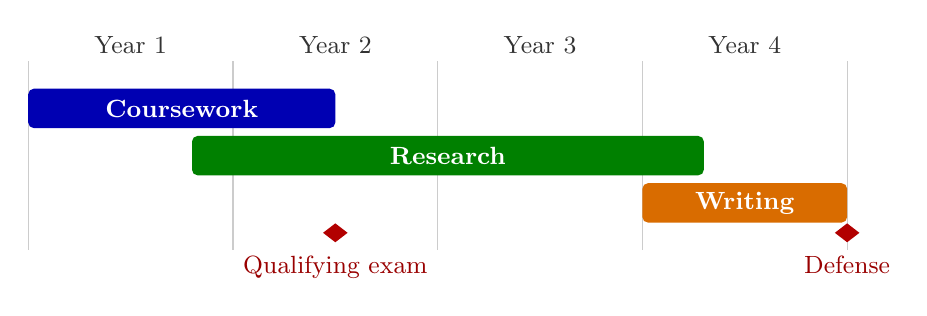
\begin{tikzpicture}[x=2.6cm, every node/.style={font=\small}, phase/.style={rounded corners=2pt, minimum height=5mm, inner sep=2pt, text=white, font=\small\bfseries}]
  \foreach \y in {0,...,4} \draw[gray!40] (\y,0.2) -- (\y,-2.2);
  \foreach \y in {1,...,4} \node[gray!40!black] at (\y-0.5,0.4) {Year \y};
  \node[phase, fill=blue!70!black, minimum width=3.9cm] at (0.75,-0.4) {Coursework};
  \node[phase, fill=green!50!black, minimum width=6.5cm] at (2.05,-1.0) {Research};
  \node[phase, fill=orange!85!black, minimum width=2.6cm] at (3.5,-1.6) {Writing};
  % Milestones as diamonds: the qualifying exam at 1.5 years, the defense at 4
  \foreach \x/\t in {1.5/Qualifying exam, 4/Defense} {
    \fill[red!70!black] (\x,-2.1) -- ++(0.06,0.12) -- ++(-0.06,0.12) -- ++(-0.06,-0.12) -- cycle;
    \node[below, red!60!black] at (\x,-2.15) {\t};
  }
\end{tikzpicture}
